\section{Zemax 物镜设计仿真与优化}

\subsection{Cousa 物镜：文献参数与优化参数对比}

\englishtitle{Cousa Objective in Zemax: Published and Optimized Prescriptions}
\begin{frame}{Cousa 物镜：文献参数与优化参数}
    \small
    \framerefbox{Yu, C.-H. et al., Nature Methods 21, 132--141 (2024). DOI: 10.1038/s41592-023-02098-1}
    \begin{columns}[T]
        \begin{column}{.49\textwidth}
            \begin{figure}
                \centering
                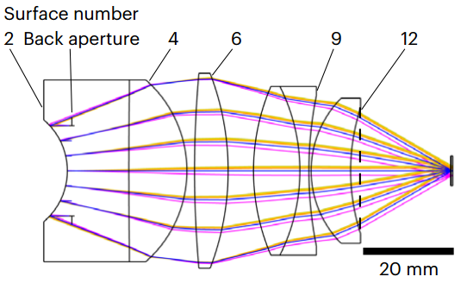
\includegraphics[width=.98\textwidth,height=.25\textheight,keepaspectratio]{Figure/ZemaxSimulation/布局图_01.png}
                \vspace{2pt}
                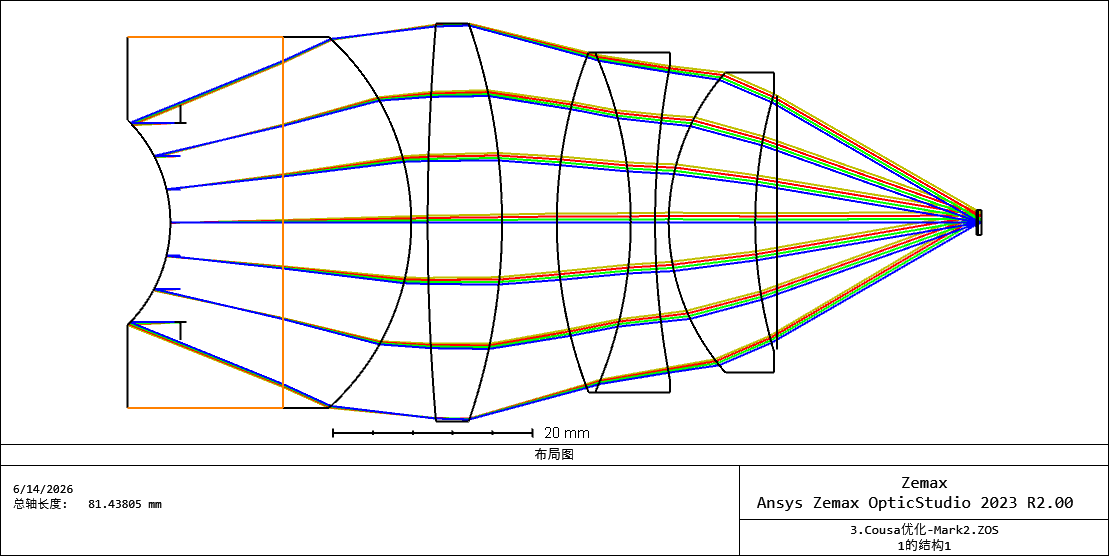
\includegraphics[width=.98\textwidth,height=.24\textheight,keepaspectratio]{Figure/ZemaxSimulation/布局图_02.png}
                \caption{上：文献参数（01）；下：我的 Zemax 优化参数（02）}
                \label{fig:cousa_layout_compare}
            \end{figure}
        \end{column}
        \hfill
        \begin{column}{.49\textwidth}
            \begin{block}{本章对比对象}
                \begin{itemize}
                    \item \textbf{01}：按文献公开参数重建的 Zemax 结果。
                    \item \textbf{02}：在同一目标下进一步优化后的参数结果。
                \end{itemize}
            \end{block}

            \begin{block}{关注的四类指标}
                \begin{itemize}
                    \item 布局图：看长工作距下的结构分配。
                    \item RMS / OTF：看像质随视场的变化。
                    \item 网格畸变：看 3$^\circ$ 与 5$^\circ$ 视场的几何失真。
                    \item 斯特列尔比：看是否维持在衍射极限附近。
                \end{itemize}
            \end{block}

            \textbf{主线问题：}在保持 Cousa 长工作距设计目标的同时，优化后的参数是否让全视场像质更均匀、可用范围更大。
        \end{column}
    \end{columns}
\end{frame}

\englishtitle{Layout Comparison}
\begin{frame}{布局图对比：在长工作距约束下重新分配像差}
    \begin{columns}[T]
        \begin{column}{.49\textwidth}
            \begin{figure}
                \centering
                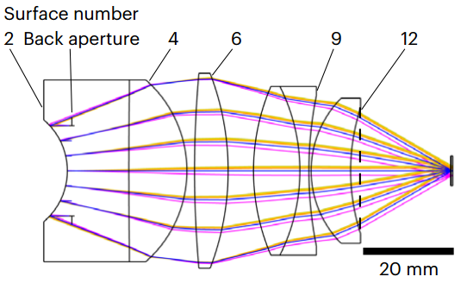
\includegraphics[width=\textwidth,height=.40\textheight,keepaspectratio]{Figure/ZemaxSimulation/布局图_01.png}
                \caption{文献参数重建结果}
                \label{fig:cousa_layout_lit}
            \end{figure}
        \end{column}
        \hfill
        \begin{column}{.49\textwidth}
            \begin{figure}
                \centering
                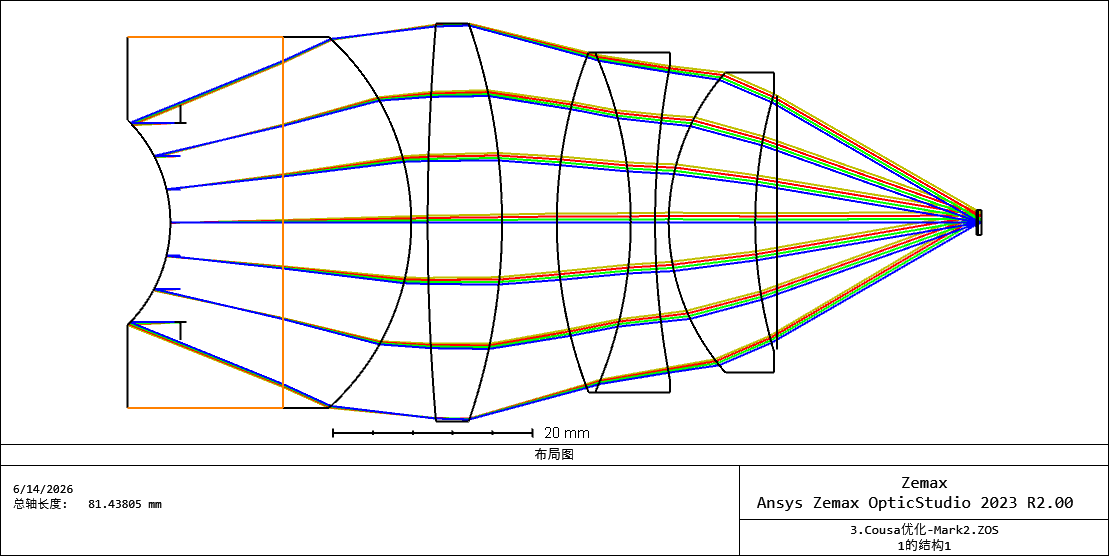
\includegraphics[width=\textwidth,height=.40\textheight,keepaspectratio]{Figure/ZemaxSimulation/布局图_02.png}
                \caption{优化后参数结果}
                \label{fig:cousa_layout_opt}
            \end{figure}
        \end{column}
    \end{columns}

    \vspace{-3pt}
    \begin{itemize}
        \item 优化并不是推翻原始 Cousa 架构，而是在相近系统边界内重新分配各组透镜承担的像差校正任务。
        \item 这种长工作距、大后工作空间的物镜，对前组口径、后组会聚角和全系统总长的耦合非常敏感。
        \item 后续 RMS、畸变和 Strehl 的变化，本质上是在检验这次结构再平衡是否真的换来了更稳的全视场表现。
    \end{itemize}
\end{frame}

\englishtitle{Wavefront Error Comparison}
\begin{frame}{RMS 波前误差：文献参数与优化参数对比}
    \begin{figure}
        \centering
        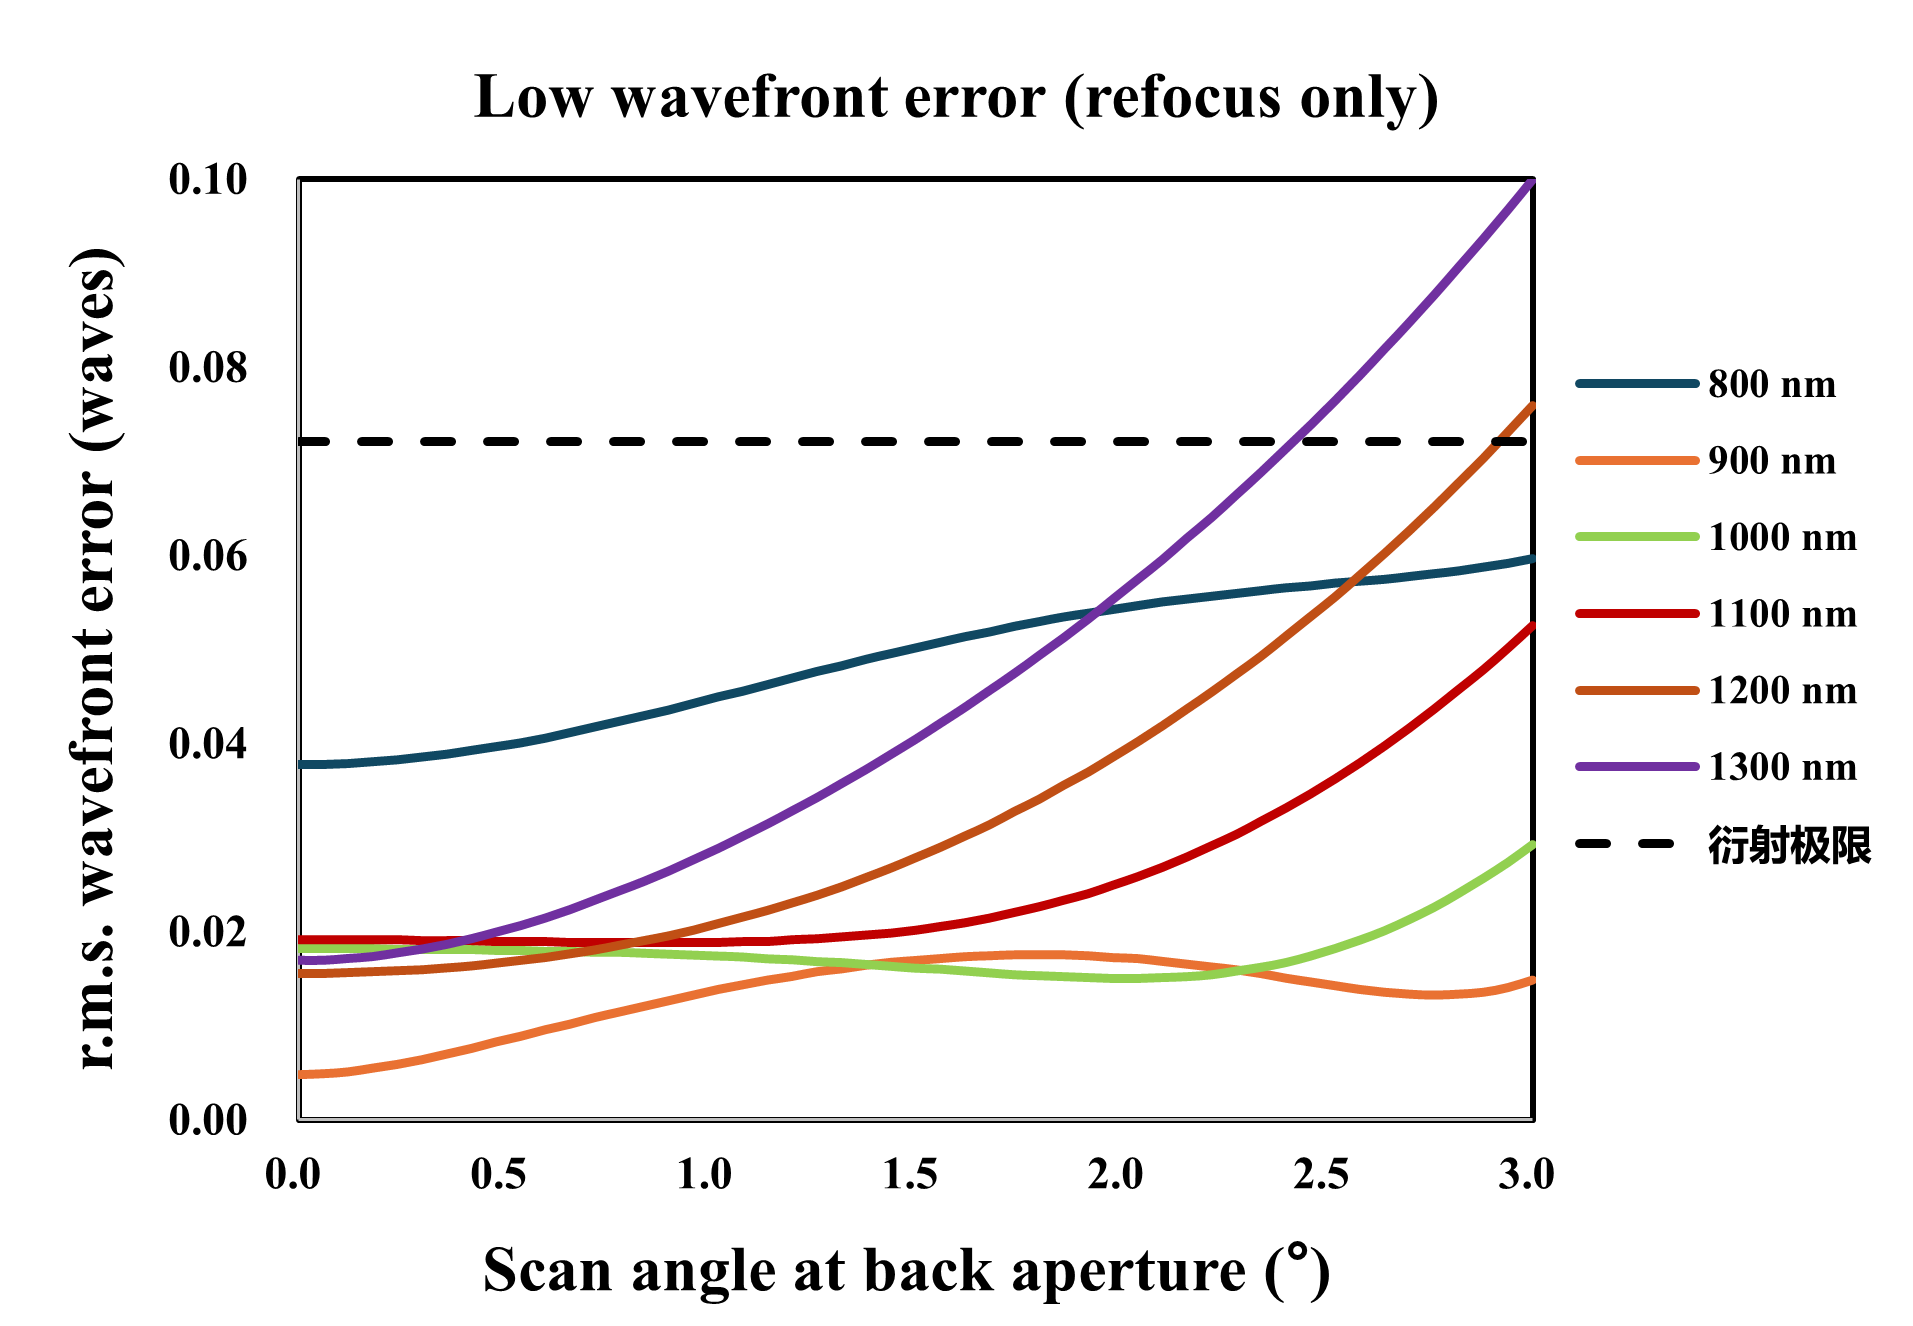
\includegraphics[width=.47\textwidth,height=.31\textheight,keepaspectratio]{Figure/ZemaxSimulation/RMS_01.png}\hfill
        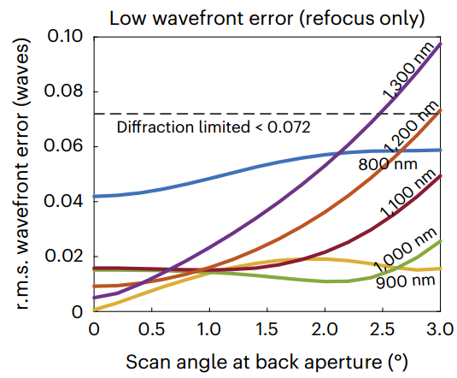
\includegraphics[width=.22\textwidth,height=.31\textheight,keepaspectratio]{Figure/ZemaxSimulation/RMS_02.png}
        \caption{左：文献参数重建的 RMS wavefront error；右：优化后参数的 RMS wavefront error}
        \label{fig:cousa_rms_compare}
    \end{figure}

    \vspace{-2pt}
    \begin{columns}[T]
        \begin{column}{.52\textwidth}
            \begin{itemize}
                \item 文献图中给出的判据是 RMS wavefront error 低于约 0.072 waves 时可视作接近衍射极限。
                \item 重建结果可以作为基准，判断 Cousa 原始公开设计在主工作视场中的误差抬升趋势。
            \end{itemize}
        \end{column}
        \begin{column}{.48\textwidth}
            \begin{itemize}
                \item 我的优化结果把主要工作波段压到更低的 RMS 水平，并让随视场增长的趋势更平缓。
                \item 这说明优化并不只是改善轴上点，而是提升了扫描过程中的全场一致性。
            \end{itemize}
        \end{column}
    \end{columns}
\end{frame}

\englishtitle{RMS and OTF Across Field}
\begin{frame}{RMS 与 OTF 随视场变化：优化后的全场表现}
    \begin{columns}[T]
        \begin{column}{.36\textwidth}
            \begin{figure}
                \centering
                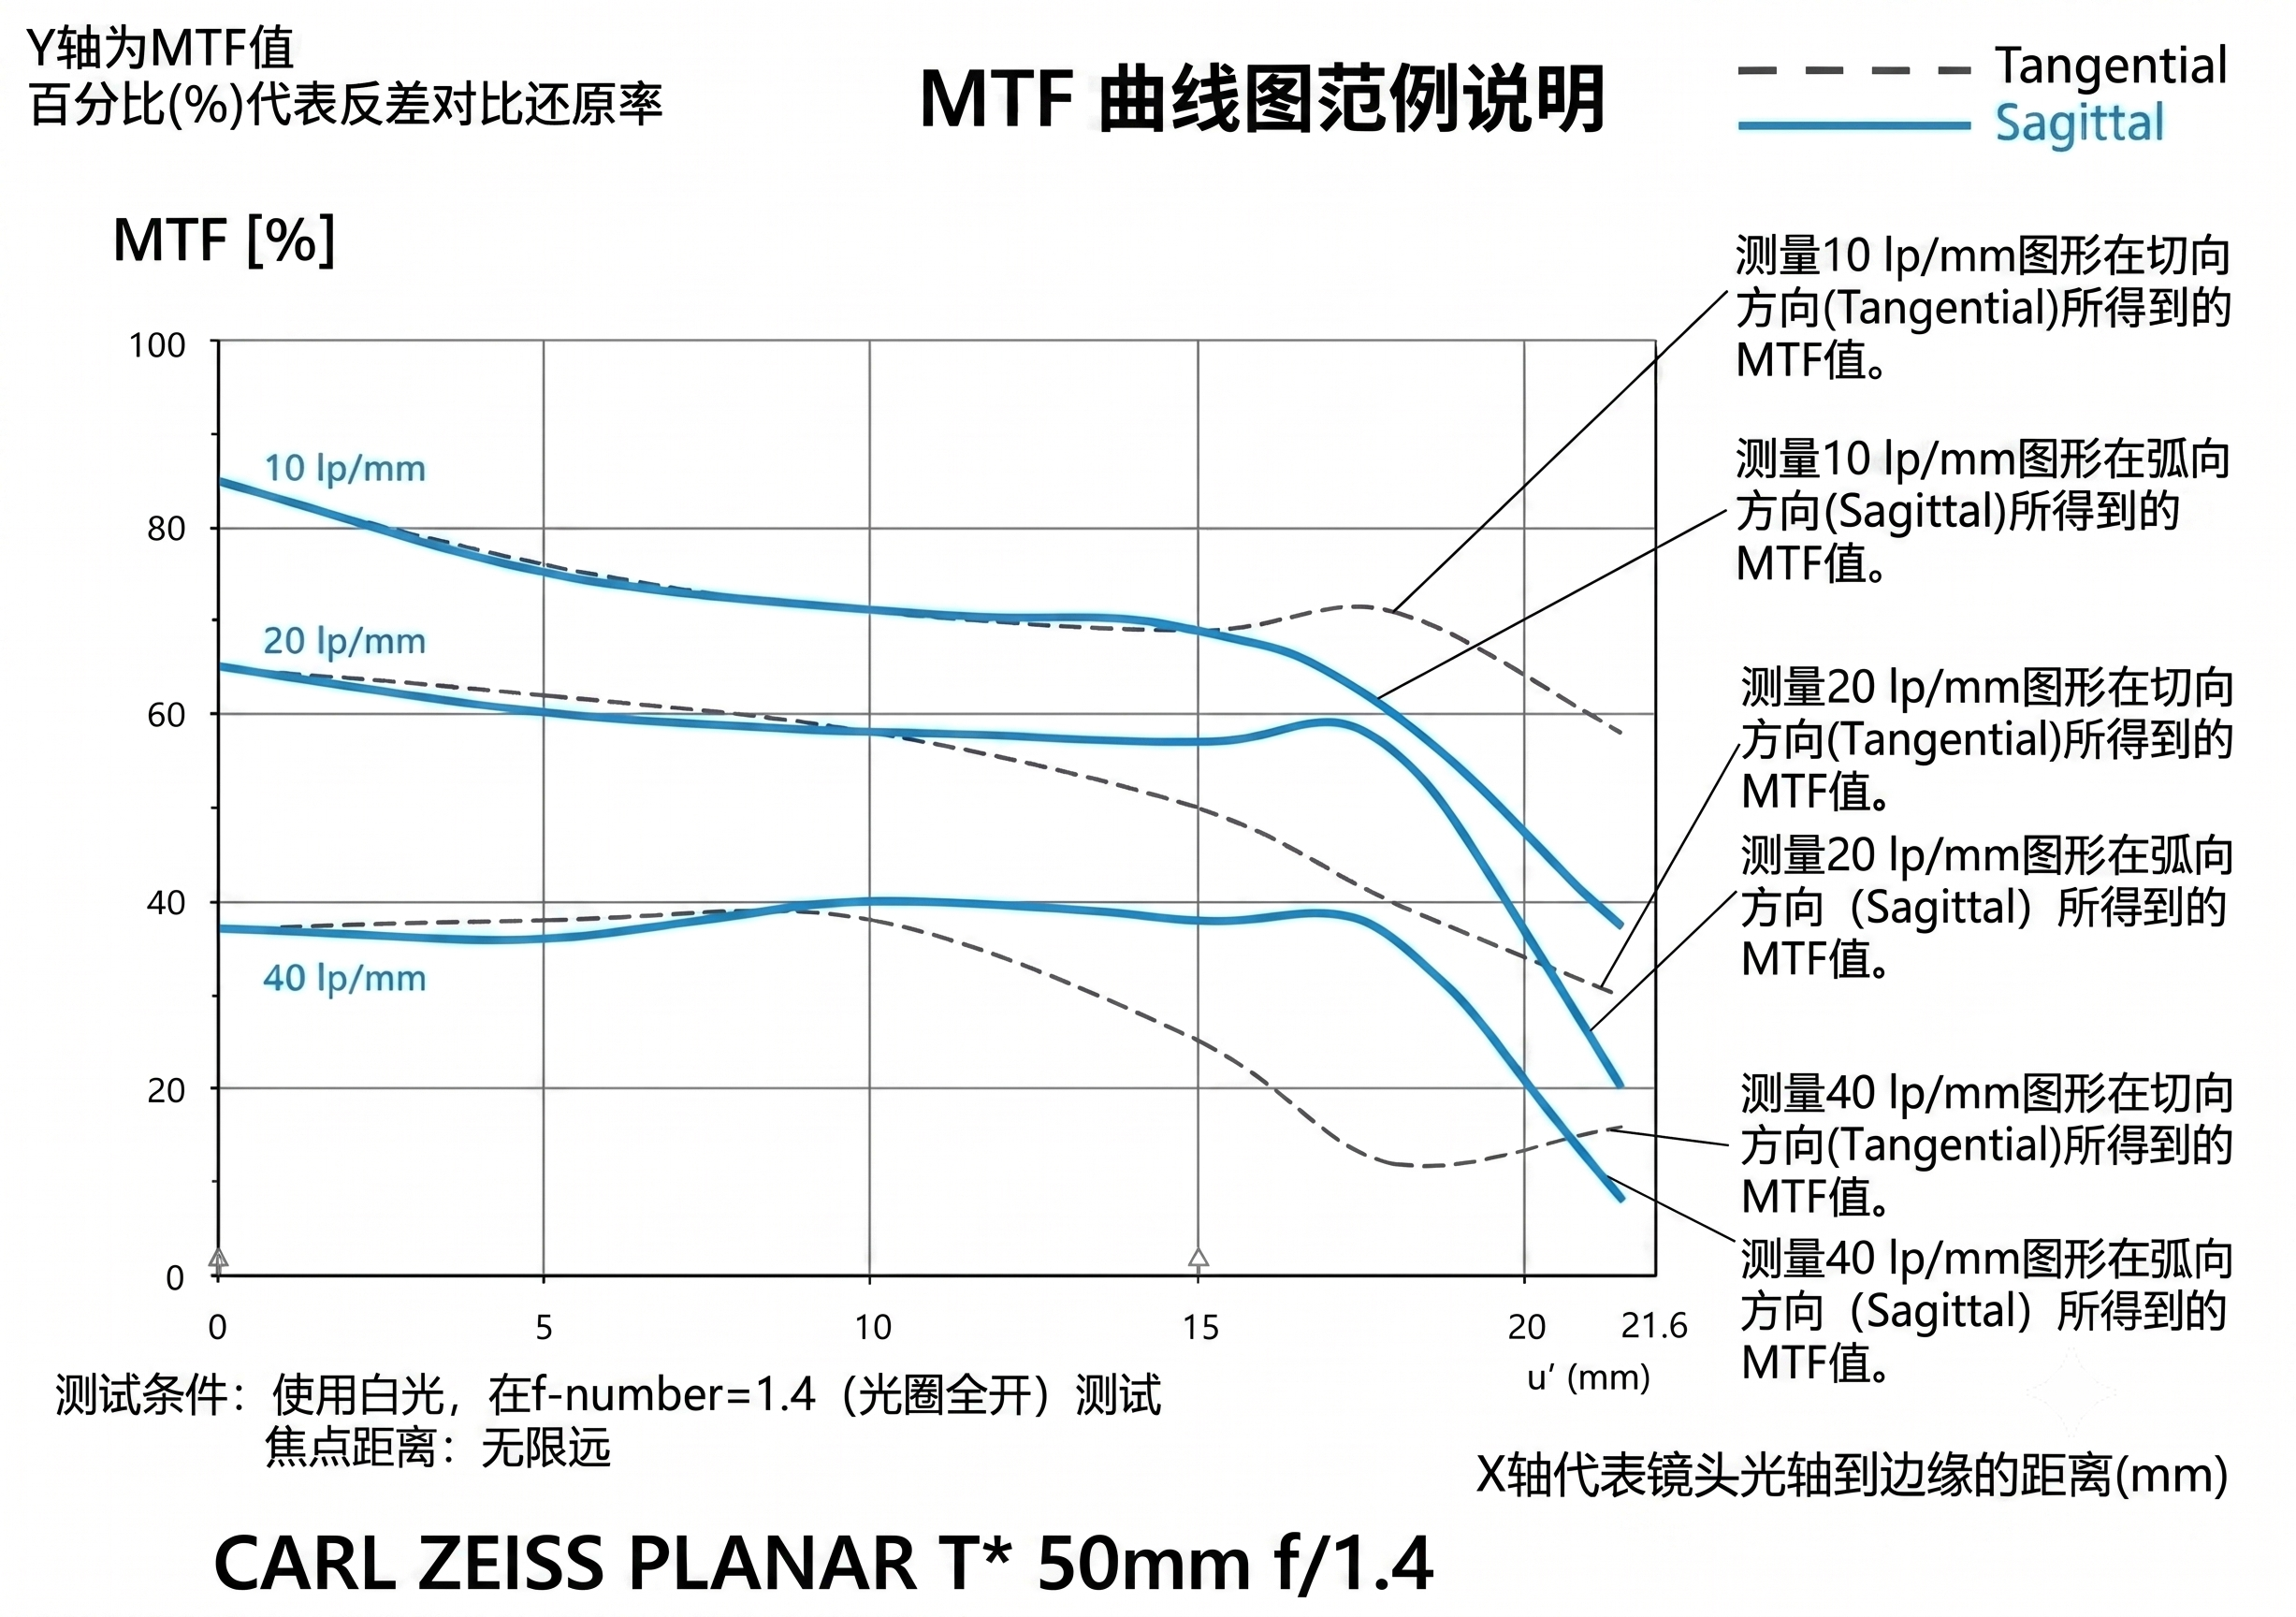
\includegraphics[width=\textwidth,height=.58\textheight,keepaspectratio]{Figure/ZemaxSimulation/MTF.png}
                \caption{MTF 曲线读法示意：切向/弧矢方向对比度传递}
                \label{fig:cousa_mtf_explain}
            \end{figure}
        \end{column}
        \hfill
        \begin{column}{.64\textwidth}
            \begin{figure}
                \centering
                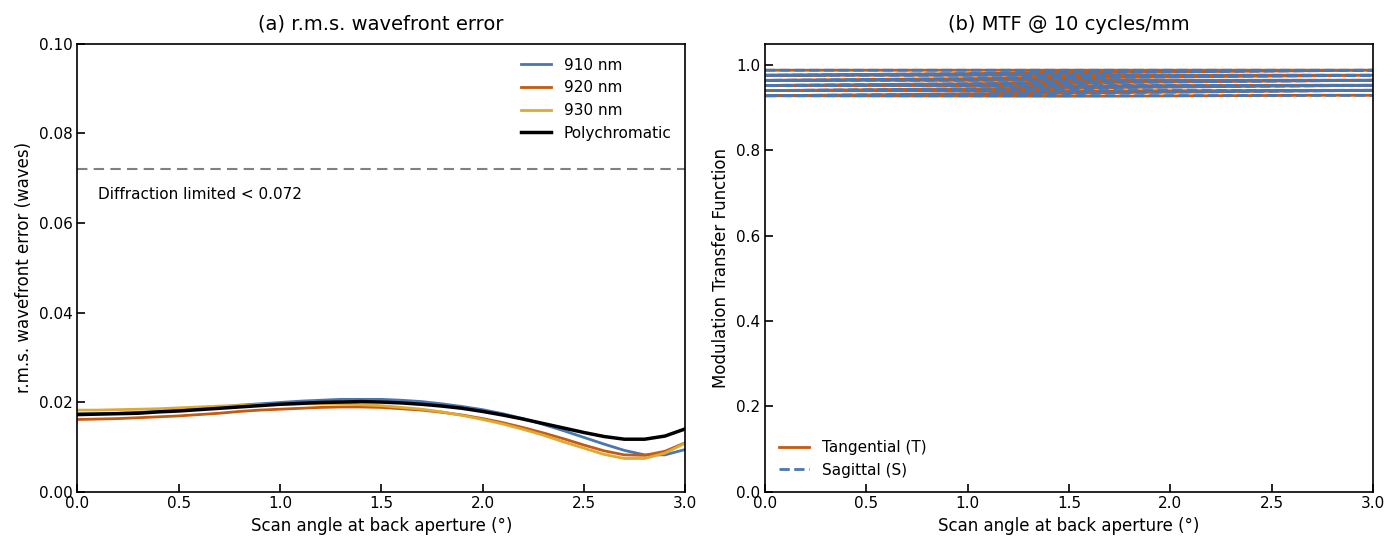
\includegraphics[width=\textwidth,height=.58\textheight,keepaspectratio]{Figure/ZemaxSimulation/RMS_03.png}
                \caption{优化后 RMS 与 10 cycles/mm OTF 随扫描视场变化}
                \label{fig:cousa_rms_otf_opt}
            \end{figure}
        \end{column}
    \end{columns}

    \vspace{-4pt}
    \begin{itemize}
        \item 左图用于说明 OTF/MTF 读图方式；右图则把优化后的波前误差和 10 cycles/mm 对比度保持能力放在同一页里。
        \item 从结果看，优化后 910/920/930 nm 三条曲线在主视场内都维持较低 RMS，切向与弧矢 OTF 也接近 1。
        \item 这意味着优化后的 Cousa 仿真不仅接近衍射极限，而且在扫描到边场时仍保持很高的低频结构还原能力。
    \end{itemize}
\end{frame}

\englishtitle{Distortion Comparison}
\begin{frame}{网格畸变：标准 3$^\circ$ 与扩展 5$^\circ$ 视场}
    \begin{columns}[T]
        \begin{column}{.50\textwidth}
            \begin{figure}
                \centering
                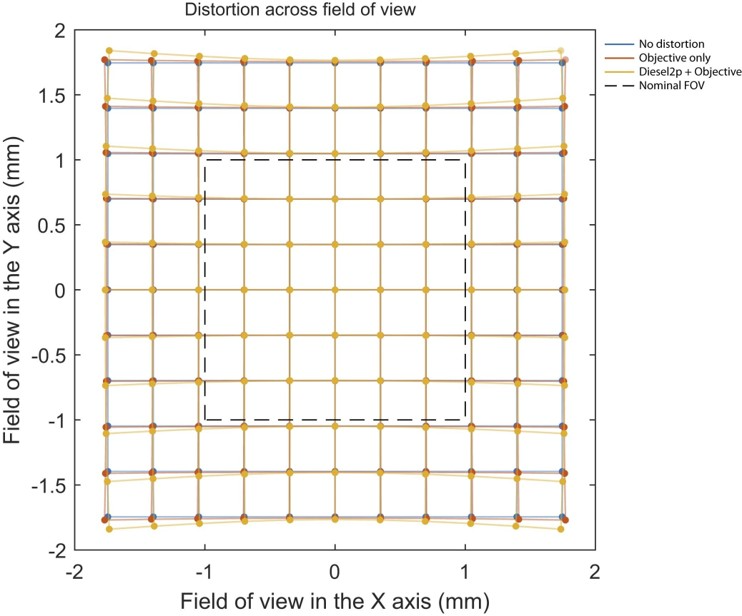
\includegraphics[width=\textwidth,height=.44\textheight,keepaspectratio]{Figure/ZemaxSimulation/网格畸变_01.png}
                \caption{文献参数重建：虚线框内为标准 3$^\circ$ 视场}
                \label{fig:cousa_distortion_lit}
            \end{figure}
        \end{column}
        \hfill
        \begin{column}{.50\textwidth}
            \begin{figure}
                \centering
                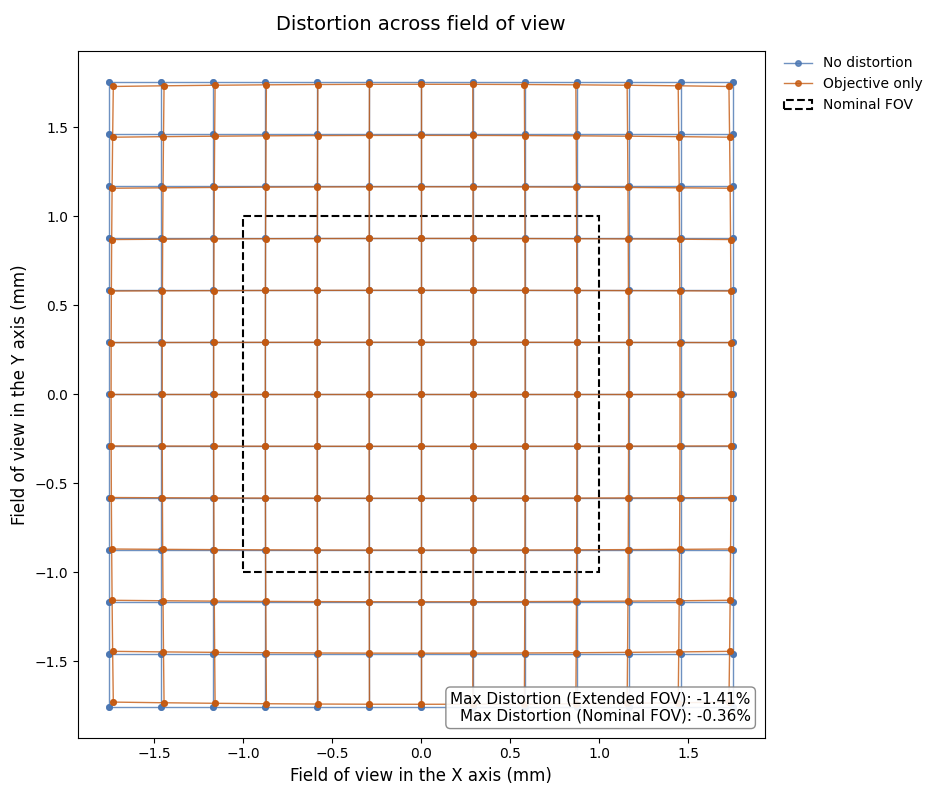
\includegraphics[width=\textwidth,height=.44\textheight,keepaspectratio]{Figure/ZemaxSimulation/网格畸变_02.png}
                \caption{优化后：5$^\circ$ 扩展视场下仍保持较低畸变}
                \label{fig:cousa_distortion_opt}
            \end{figure}
        \end{column}
    \end{columns}

    \vspace{-4pt}
    \begin{itemize}
        \item 虚线框表示标准 3$^\circ$ 扫描工作区，框外则对应更大的扩展视场评估。
        \item 优化后图中已直接给出数值：标准视场最大畸变约为 0.36\%，扩展 5$^\circ$ 视场最大畸变约为 1.41\%。
        \item 这个结果说明优化后的参数不只是在中心场更好，也把大视场扫描时的几何一致性控制在较可用的水平。
    \end{itemize}
\end{frame}

\englishtitle{Strehl Ratio Comparison}
\begin{frame}{斯特列尔比：是否稳定维持在衍射极限附近}
    \begin{columns}[T]
        \begin{column}{.34\textwidth}
            \begin{figure}
                \centering
                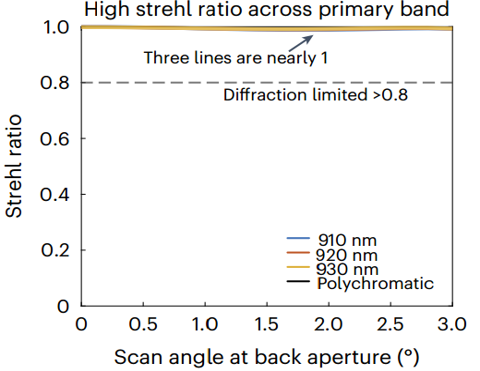
\includegraphics[width=\textwidth,height=.46\textheight,keepaspectratio]{Figure/ZemaxSimulation/斯特列尔比_01.png}
                \caption{文献参数重建结果}
                \label{fig:cousa_strehl_lit}
            \end{figure}
        \end{column}
        \hfill
        \begin{column}{.66\textwidth}
            \begin{figure}
                \centering
                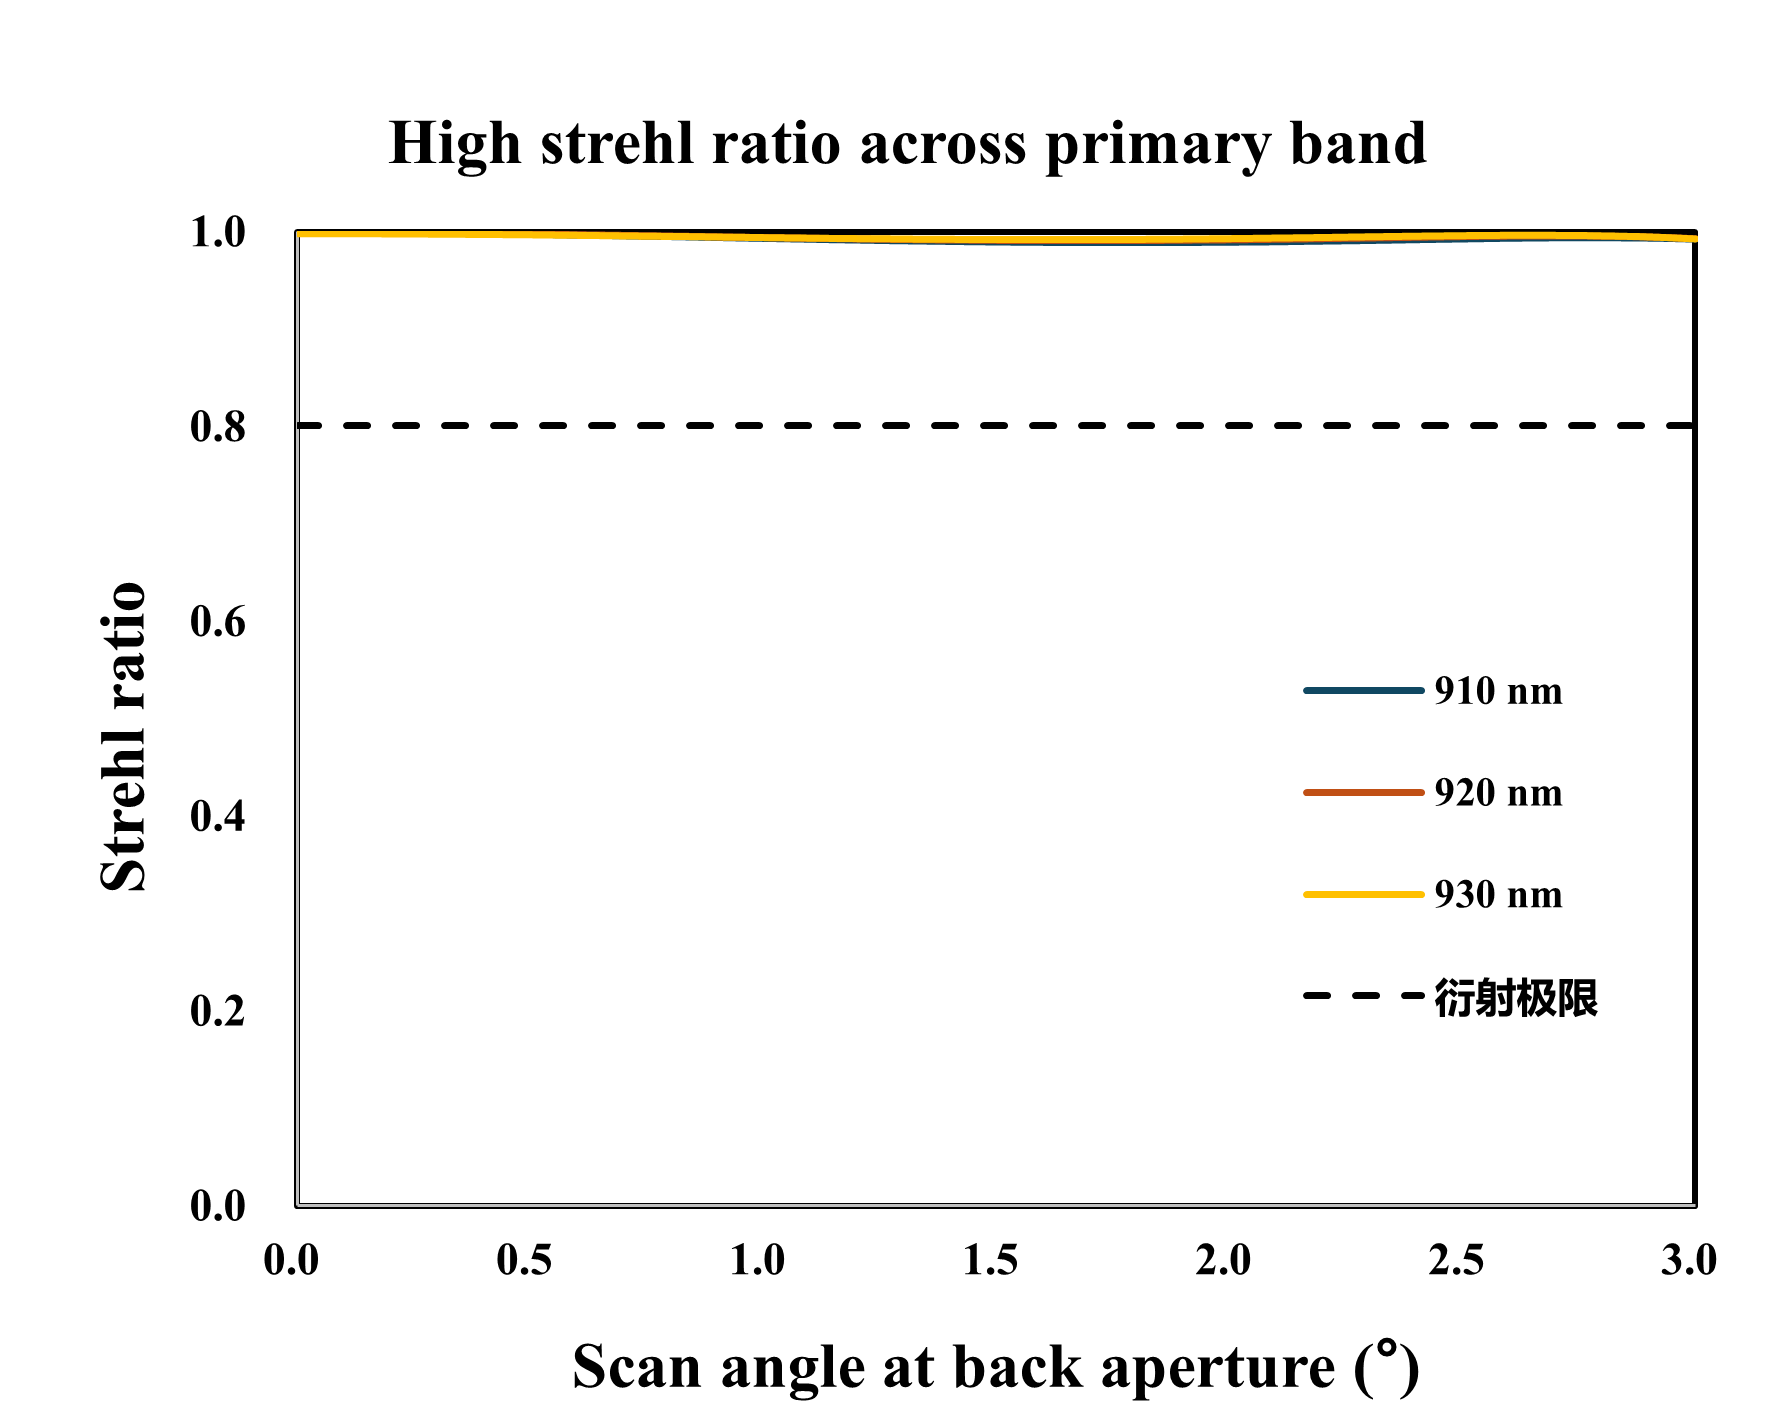
\includegraphics[width=\textwidth,height=.46\textheight,keepaspectratio]{Figure/ZemaxSimulation/斯特列尔比_02.png}
                \caption{优化后结果：主工作波段的 Strehl 几乎贴近 1}
                \label{fig:cousa_strehl_opt}
            \end{figure}
        \end{column}
    \end{columns}

    \vspace{-5pt}
    \begin{itemize}
        \item Strehl ratio 高于 0.8 通常可视作达到衍射极限附近；而优化后的三条工作波长曲线几乎都贴近 1。
        \item 这和前面的低 RMS、接近 1 的 OTF 是一致的，说明优化后的 Cousa 设计在主视场内具备很强的波前保真度。
        \item 对长工作距多光子物镜来说，这一点尤其重要，因为它意味着放宽机械空间后并没有明显牺牲主视场的像质上限。
    \end{itemize}
\end{frame}
